\documentclass{article}

\setlength{\parskip}{10pt}

\title{Literature Review for AI Solutions for Training Scenarios for High-pressure Situations}
\author{Richard Lay-Flurrie}

\usepackage{cite}
\usepackage{soul}
\usepackage{xcolor}
\usepackage{graphicx}

\begin{document}

\maketitle

\tableofcontents

% Begin %

% Introduction %
\section{Introduction}

\subsection{The Importance of Training for Stressful Scenarios}

Every day, professionals all over the world are put into stressful situations in which they have to make decisions, often very quickly, which can have deadly consequences \hl{(Find example)}. The consequences of the wrong decision(s) being made can be tragic(https://web.archive.org/web/20100522064638/http://www.freep.com/article/20100519/NEWS01/5190356/0/BUSINESS06). Training for these scenarios is normally conducted by carrying out real life exercises but these generally face limitations such as cost, logistics issues and scope of the scenarios available \hl{(Use that forces news report about the cost of ammo)}.

\subsection{Software for Training}

The flexibility of software-based simulations is unmatched \hl{(Find example)} and the call for its inclusion in training for stressful situations is very real \hl{(Find example)}. However, these scenarios are often generated by people, with a specific training goal in mind, which can impact the training scenario's utility in training personnel for organic/dynamic situations they may face for real in '\hl{the field}'. A potential solution to this limitation, is to provide AI-generated training scenarios, in which no one participant is aware of the parameters of the scenario, enabling them to focus entirely on solving evolving problems and completing dynamic tasks in the simulation.

One major limitation of the simulation of stressful scenarios is the disconnect between simulation and reality in terms of \hl{stress levels} affecting the performance of the participant. For example, one may be able to defuse a bomb in a simulation 10 times out of 10. However, if you then put that participant in the same situation but for real, the fear of injury or death through detonation may cause the participant to behave differently, resulting in an unsafe procedure.

\begin{figure}[ht]
    \centering
    \begin{minipage}[b]{0.9\linewidth}
      
\includegraphics[width=\linewidth]{Images/cheeseMeister3kMario.png}
      \caption{"Mario games teach us that even if something is essentially the same, psychologically it can be completely different. This example is very easy to understand." - Cheesemeister3k on X (\hl{https://twitter.com/Cheesemeister3k/status/1547440825420099586})}
      \label{fig:image1}
    \end{minipage}
  \end{figure}

With the sudden rise in popularity of AI tools such as ChatGPT, many people and organisations now have an accessible route into the world of artificial intelligence and are now exploring ways to incorporate it into their metaphorical toolkit \hl{Talk about Amy's work}. 

\subsection{How Recent is the Simulation of Stressful Scenarios?}

The use of simulation, for the purposes of entertainment and training has been prevalent for hundreds of years \hl{Really?}, with examples of software for simulation dating back to 1947 (https://patents.google.com/patent/US2455992) and documentation of simulated battles for training going as far back as at least 1824 (general von muffling), as well as examples for medical education going back to the late 1700s (https://www.ncbi.nlm.nih.gov/books/NBK559082/). The earliest potential example of an attempt at simulation for entertainment \hl{(discounting people role-playing in play)} is a board game called Senet, dating back to 2620 BCE (https://journals.sagepub.com/doi/epub/10.1177/0307513319896288).


  \subsection{Research Question\hl{(s?)}}
  
  Generating AI-driven scenarios for realistic small-unit training scenarios. 
  
  \hl{Hypothesis}
  
  It is possible to produce a scenario in a simulated environment, in which self-preservation is paramount to the user, with the help of AI.
  
  
  \section{Defining Terms}

  \subsection{What is a High-pressure Situation?}

  Pressure can be defined as "stress or anxiety that an individual feels as a result of external or internal demands or expectations". (https://www.psychology-lexicon.com/cms/glossary/49-glossary-p/15234-pressure.html)

  "psychological stress exceeding certain intensity affects the quality of decision making" % https://psycnet.apa.org/doiLanding?doi=10.1037%2F0022-3514.52.3.639 %
    
  % https://www.reddit.com/r/GlobalOffensive/comments/1ak7n2j/for_research_can_you_describe_that_feeling_you/ %

      % https://www.tandfonline.com/doi/abs/10.1080/12460125.2020.1768680?casa_token=mB4eZQrxMkgAAAAA:bjOHSmi1NrMYMLYCOXvw4hxArJDSsypa9CGWEFkL7upxRr-4yg0PYKpZM5Gm92xZcEevhCcMWbIbZQ %

      \subsection{Decision Stressors}

      - Information Overload
      - Time Pressure
      - Complexity
      - Uncertainty and risk

      \subsection{Further Decision Stressors}

      - Fear of Missing Out
      - Fear of Bad First Impression
      - Competition


  \subsection{Is it Really Stress?}

  Stress can be defined as "a state of worry or mental tension caused by a difficult situation" 

  %https://www.who.int/news-room/questions-and-answers/item/stress#:~:text=Stress%20can%20be%20defined%20as,experiences%20stress%20to%20some%20degree.%

  \subsection{What is Duress?}

  From Oxford Languages, "threats, violence, constraints, or other action used to coerce someone into doing something against their will or better judgement." However, it appears as though duress is commonly used specifically in the context of someone committing a crime because they were under fear of these consequences, rather than making a decision in a dangerous situation \hl{(Show some examples)}.

  Is it really anxiety?


  \subsection{What is Fight-or-flight?}

  From Oxford Languages, "the instinctive physiological response to a threatening situation, which readies one either to resist forcible or to run away".

  % https://www.health.harvard.edu/staying-healthy/understanding-the-stress-response %

  Acute stress

  What causes the lack of decision making ability when stressed? Adrenaline? Fear? What's the difference?



  Talk about having loss on control of the situation taken away, for example those drivers who drive the back end of the fire engine on the long ones in the US. \hl{It's called a tiller apparently.}




Talk about walking into a building in an Arma 3 PVP vs commanding the team

"Next 15 seconds are decisive" - Talk about how this matches what the tiller operator has to do

What about when you know you are going to lose? The feeling immediately goes away. 

Fear of the unknown.

Does there need to be a win/lose scenario? 

People when they die in game immediately get their phone out and go on TikTok or Youtube Shorts.

You want to try and outsmart your equals or superiors. Sneaking up on someone in a game or making them fall for it.

\section{Types of Computer Software used in Simulation}

Simulation 4.0 \cite{DEPAULAFERREIRA2020106868}

\begin{itemize}
    \item Agent-based Modelling and Simulation (ABMS)
    \item Artificial Intelligence (AI)
    \item Augmented Reality (AR)
    \item Continuous Simulation
    \item Digital Twins (DT)
    \item Discrete Event Simulation (DES)
    \item Hybrid Simulation (HS)
    \item Petri Nets Simulation (PN)
    \item Virtual Commissioning (VC)
    \item Virtual Reality (VR)    
    \item System Dynamics (SD)    
\end{itemize}

\subsection{Agent-based Modelling and Simulation (ABMS)}

Agent-based modelling and simulation consists of modelling systems by making use of autonomous agents interacting with one another. \cite{1574234}

\subsection{Artificial Intelligence (AI)}

Artificial intelligence is a simulation of a thinking being's capability to perform cognitive functions such as decision making, reasoning, seeing and communicating.

% https://www.mdpi.com/2673-2688/1/2/8 %

\hl{Talk about what this means in comparison to technology such as cassette-based car navigation. Use the clip from Tomorrow's World: https://www.bbc.co.uk/archive/cassette-based-navigation-1971/z6sbt39}

"There is one drawback in all this, though, if for some reason or another the road system has been altered, there are roadworks or some diversion in force, which isn't programmed on the tape, well then this whole business just becomes one glorious guided mystery tour."

\hl{Is Google Maps AI?}

Contrast this with the capabilities of Google Maps in which a diversion is handled well in almost every instance.

\subsection{Augmented Reality (AR)}

Augmented reality is a combination of real-world and computer-generated audio and visual, typically provided by software on a mobile device with a screen such as a smartphone, glasses or laptop. The user views the real world through the device's camera setup, with visuals laid over the image making them appear as if they were present in the real world.

A recent, high-profile addition to this is Apple's vision...



\subsection{Mixed Reality (MR)}

% Apple Vision Pro %

Are Snapchat filters mixed or augmented reality?

\subsection{Extended Reality (XR)}

Extended reality is a term which refers to augmented reality, mixed reality and virtual reality. 

\subsection{Digital Twins (DT)}

A digital twin can be defined as "a dynamic virtual representation of a physical object or system, usually across multiple stages of its lifecycle. It uses real-world data, simulation or machine learning models, combined with data analysis, to enable understanding, learning, and reasoning" \cite{stanford2019digital}. 

Their use spans a wide range of disciplines including manufacturing, automotive, energy \cite{PYLIANIDIS2021105942}
 and training applications for emergency services \cite{ScientificReports1} and military personnel \cite{9345490}. 

\subsection{Continuous Simulation}

% https://proceedings.systemdynamics.org/2009/proceed/papers/P1199.pdf %

\begin{itemize}
  \item Vehicle modelling such as steering, breaking and accelerating
\end{itemize}

\subsection{Discrete Event Simulation (DES)}

% Look at SimPy: https://simpy.readthedocs.io/en/latest/ %

% https://www.ncbi.nlm.nih.gov/books/NBK293948/ %

Discrete Event Simulation (DES) provides a method for testing "what if?" scenarios by simulating the "behaviour and performance of a real-life process, facility or system". [https://www.ncbi.nlm.nih.gov/books/NBK293948/] DES provides a model by simulating a series of events. For example, 

\begin{itemize}
  \item Queueing Simulations such as plane boarding
  \item Livestock management
\end{itemize}

"It's this technique of mixing determinism and non-determinism, that makes DES so valuable" \footnote{https://www.oreilly.com/library/view/sql-in-a/9780596155322/ch04s01s01.html} (MATLAB YOUTUBE VIDEO)

%https://www.youtube.com/watch?v=3EiniZbyeV0&ab_channel=MATLAB%

\subsection{Hybrid Simulation}


\hl{Talk about sensory deprevation tanks and the possibility of using VR in combination with that}

\hl{"If you were to overlay a virtual reality scenario into that situation you would have no stimulus to counteract what your eyes are seeing." Sam}

\section{Stressful Scenarios}

\subsection{Driving Tests}

%Why are they so stressful? How can this feeling be replicated in training?

My own anecdote: 

During my final attempt at a driving test, I was incredibly nervous. I then made an error which I thought was a test fail. As I thought I had failed, my nerves all went and I found the rest of the test very easy.

\section{Software-based Simulation of Stressful Situations}

\subsection{Introduction}

When humans make decisions, this process can be impacted by factors such as oxygen levels [] and stress[].

% Oxygen Levels %
% https://www.cambridge.org/core/journals/judgment-and-decision-making/article/decision-making-under-hypoxia-oxygen-depletion-increases-risk-seeking-for-losses-but-not-for-gains/29B6B25680FDACB70A8F518E6D67BD00 %

% Stress %
% https://www.ncbi.nlm.nih.gov/pmc/articles/PMC5201132/ %

% Difference between long term and short term stress %
% https://www.ncbi.nlm.nih.gov/pmc/articles/PMC5964013/#:~:text=Short%2Dterm%20stress%20has%20been,weeks%20or%20months%20%5B9%5D. %

%https://www.port.ac.uk/study/postgraduate-research/research-degrees/phd/explore-our-projects/the-effects-of-hypoxia-on-decision-making-cognitive-flexibility-memory-and-pain#:~:text=Individuals%20may%20be%20placed%20in,this%20link%20is%20not%20known.%
%https://link.springer.com/article/10.1007/s10111-015-0325-3%

\subsection{Cyber Attacks}

\subsection{Diving}

\hl{Talk about diving in Arma 3}

\hl{Talk about how nice conditions can be dangerous because you can "forget" where you are}

\subsection{Finance}

\subsubsection{Monte Carlo Simulation}


\subsection{Medicine}

% https://academic.oup.com/ageing/article/49/2/270/5679684 %

The field of medicine makes great use of simulation in areas such as training for surgery  and estimating the impact of certain health conditions on society. Discrete Event Simulation provided means for estimating the societal cost of stroke \hl{FOOTNOTE} cases in the UK for 2014/2015. \cite{afz162}

\subsection{Emergency Services}

\subsubsection{Firefighting with Aircraft}

According to the Emergency Management Professionalisation Scheme of Australia and New Zealand, an Air Attack Supervisor (AAS) is an individual who is "responsible for for supervising aerial fire suppression activities and other tactical missions from the air". \hl{TODO:}

% https://www.emps.org.au/wp-content/uploads/2021/12/EMPSProfStandard_Registered_Air_Attack_Supervisor_web.pdf %

A 2019 study found that virtual reality training exercises produce stress levels which are similar to those of a real exercise, when measured by heart rate variability (HRV). \cite{8797889}

\hl{TODO:} Talk about how this may be because AAS applicants are already experienced pilots.

\subsubsection{Measuring Stress Levels of Participants in Simulated Scenarios}

Data regarding the stress level of a participant can be taken by observing their heart rate, heart rate variability (HRV), how fast they are breathing, eye movement and chemical measurements. \cite{8797889}

\section{Simulation}

\subsection{Difference Between Simulation and Role-play}



\subsection{What is Military Simulation?}

"This is not a game! This is training for war! I must recommend it to the whole Army." - General von Muffling, Prussian Staff Officer, 1824.

\subsubsection{Combined Arms Tactical Trainer}

% https://www.youtube.com/watch?v=TNfc90Zs5co %

% Contact for placements/work experience %

% RG-NRCOutreachAdmin@mod.gov.uk %

\subsection{What is it used for?}

\hl{Military simulation/simulation of stressful scenarios} are used for leisure, training and prediction of possible outcomes of real-life stressful scenarios.

\hl{This can be seen in entertainment with examples such as..., training with examples such as... and predictions with examples such as... .}

\subsection{How Accurate are (Military) Simulations?}

Military simulation software is designed to accurately replicate real life performance of \hl{things} (\hl{TODO: Thing? Really? That's the word you came up with?}), such as the performance of weapon systems, vehicles and other technology commonly found in the \hl{battlespace (TODO: Define this as it's not an intuitive term)}.\footnote{Test here talk about battlespace} Some simulators also go as far as to model the performance of humans in terms of physical performance, health and awareness (\hl{TODO: Expand on this}).

However, a common experience from users is often that the majority of simulators that they play feel extremely realistic, yet perform differently when compared to each other. How can two simulators be realistic if they perform differently? (\hl{TODO: This is entirely my experience and some friends I know have said this. Maybe this is a research project to carry out?})

\subsubsection{Destruction of Russian T-90 Proryv}

On the 13th of January, 2024, the 47th Separate Mechanized Brigade of the Ukrainian Army reported the destruction of a Russian T-90 Proryv tank. TODO: [] While, as of 23/01/24, not all of the details have been confirmed about the engagement, it has been proven that the T-90's external systems (such as optics) were destroyed by the main cannon of a Bradley AFV, commanded by Serhiy of the Ukrainian Army. In an interview with SerhiyTODO:[], he stated that he knew which parts of the tank to fire at (to damage the external systems) as he had practised in "video games" (it is likely, although unconfirmed, that he is referring to War Thunder TODO:[]). The translation has been independently verified by Ukrainian speakers.

In War Thunder, engagements generally take place in which another player-controlled vehicle is also trying to destroy your vehicle.


%Interview with Bradley crew from 47th Brigade https://www.youtube.com/watch?v=w_wGNqBHO4w %
%Gunner's name Serhiy
%Driver's name Oleksandr
%Gunner says that he knew where to fire because of video games [War Thunder]

\subsubsection{Influence of Music while Driving test in Simulator}

% https://ieeexplore.ieee.org/abstract/document/6294296?casa_token=aszKmSD4HEUAAAAA:LAZ8BTuIESZeTm0cNDgzsJ4jdtKj56H1Qu5-GMbfIxFXHGyD6PPJ7KSBW67vBHMDIAo_Ctcixg %

\subsubsection{World of Warcraft Virus Outbreak}

Between September 13th and October 8th 2005, players fighting a boss called Hakkar the Soulflayer could receive an in-game debuff to their characters which would spread to other characters if they were in close proximity. It was intended for this to remain only as a feature in the boss fight. However, an oversight allowed for this effect to be transferred outside in the "main" areas of the game, quickly causing this effect to spread through the characters like a virus. 

% https://www.zmescience.com/feature-post/pieces/the-weird-world-of-warcraft-pandemic-of-2005/ %

Comparisons were made between the Corrupted Blood incident and how diseases spread in real life.

\subsubsection{Top Gear Honda NSX Leguna Seca}

"Fernando Alonzo arrived there saying "Well I know my around this brand new track because I've done it on an 'x-play-box-station' or whatever it was okay and I thought "that's odd". Can you really learn your way round a racetrack on a playstation thing?" - Jeremy Clarkson for Top Gear Series 7 Episode 6.

In this episode, Jeremy Clarkson completes a lab of the race track, Leguna Seca, in the racing software Grant Turismo 4, using a digital twin of the Honda NSX. His plan is to then try and repeat this attempt in real life at the real location with a real Honda NSX.

% https://www.bbc.co.uk/iplayer/episode/b0074g6l/top-gear-series-7-episode-6?seriesId=b007gh9t %
% Timestamp 48:30 %

1'41.148 was his time on the Playstation.

"Piece of cake. But here's the thing. Could I now get round that track in that time in that car, for real?"

"This is the difference. Not sitting on a sofa [intelligible]. So that's the other thing you can do in the game is you can adjust your throttle and your breaks in the middle of a corner. You try doing that in real life, you're off. Off, wall, dead. Murder, blood, spurt, gush, artery, court-case."

2'01 was his time for real. 

An on-circuit instructor helped Jeremy Clarkson to understand where the game was "true to life" and where it was "leading him astray".

"You don't get that on a Playstation, that surge of adrenaline." 

When talking about attacking the "corkscrew" in real life in the same manner as he would in the game, Jeremy Clarkson stated that "the reality was just too daunting". 

"So much you don't feel, that G-force that you get."

After his second attempt, 1'59. 

On commenting that the brakes were "burning", Jeremy Clarkson states that it's "not me (him) that, it's the car's let me down". 

"It's that part of your brain that makes you frightened. That's what racing drivers don't have... They're not thinking "what if a wheel falls off now." "What if I push the brake pedal and nothing happens"... "and that's what I'm thinking all the time".... "What if, what if, what if."".

1'57 the final time.

\subsection{From Top Gear to Top Gun}

In the film, Tom Gun: Maverick, during a scene in which a training exercise to prepare for combat operations is depicted, three aircraft are being used to practice aerial combat. 

One character says "What say we put some skin in the game?" to which the instructor relies "What do you have in mind?".

The first character replies "Whoever gets shot down first has to do 200 push-ups". The next sequences are filmed in a way as to portray an increased sense of desire to "win" the training exercise. 

% Talk about this %

The instructor follows through and enforces the rule, ensuring the "losers" do their 200 push-ups.

In the training exercise, a kill is simulated by one aircraft locking on to another.

% Expand this %

\subsubsection{Treating Social Anxiety Disorder with VR}

\subsubsection{Training Taser with VR (AXON)}

% https://uk.axon.com/training/vr %

"It's a whole new level. You know, your heart rate gets pounding. You feel emotionally invested. You start sweating and you really feel that stress and that realism that you would in that situation"

"I have never seen the sort of intense demand that we're seeing for virtual reality training." - Rick Smith AXON CEO and Founder.

% (https://www.youtube.com/watch?v=Dvbp9ihzB2k&ab_channel=Axon) %

\subsection{AI Adversarial Command and Control}

\hl{TODO: Is the following even true or am I imagining it?}

\hl{TODO: Write about how the AI knows everything but pretends it doesn't.}

\hl{TODO: Write about developing AI which reacts to information which is only gathered the "Real way" through command and control}

\section{Computer Science Approaches to Improving Military Simulation}

\section{Types of Simulation Software}

\subsection{Bespoke vs Off the Shelf}

Two main types of simulation software appear, those which provide almost complete control over your simulated environments but require a lot of work to achieve results and those which provide limited control over your simulated environments, with the benefit of being able to put together scenarios quickly and at scale.

Two examples of these are Unreal Engine and Arma. The latest major releases of each are Unreal Engine 5 and Arma 3 \footnote{A newer release, Arma Reforger is available but does not yet feature easily accessible tools for building your own permanent simulation environments. A user can build an environment using the Game Master feature but it is wiped when the game is closed unless substantial understanding of game engines and/or server management is had by the user.}, respectively.

\subsection{Unreal Engine 5}

Unreal Engine 5 allows the user to generate basically anything they can think of within the realm of a virtual environment. However, the skills and experience necessary to do this often act as a barrier

\subsection{Unreal Engine 5 for Machine Learning Task}

As a student at the University of Essex, I was fortunate to have the opportunity to work as a research assistant, working on a machine learning task for a company called CONFIRM COMPANY NAME. 

The task involved generating synthetic data to bolster existing training data to determine whether the synthetic data could be used to improve the accuracy of the model when applied to real data. 

\subsubsection{Creating the Environment}

For this task, a landscape was created with an ocean placed on top of it. 

The landscape was then set to a specific shape with a heightmap.

Used Lumen lighting to fill the environment with light.

\subsubsection{The Buoys}

Buoy 3D models were imported with their elements being combined to make a static mesh of each buoy.

Textures were applied in the form of materials.

Buoyancy was added to the buoys by simulating pontoons, positioned as to provide realistic floatation.


\subsubsection{Taking Pictures}

To generate the images we:

Get the location of the buoy. 

Move the camera to x distance away. 

Roll, pitch and yaw the camera between set parameters. 

Take the picture.

\subsubsection{Bounding Boxes}

Shoot a bunch of "lasers" at the buoy.

Get the ones which are furthest apart, top, right, bottom, left.

Draw a line through each one. 

Run this on each frame to keep the bounding box updated.

\subsubsection{Masks}

Use the layer system. 

\begin{figure}[h]
  \centering
  \begin{minipage}[b]{0.9\linewidth}
    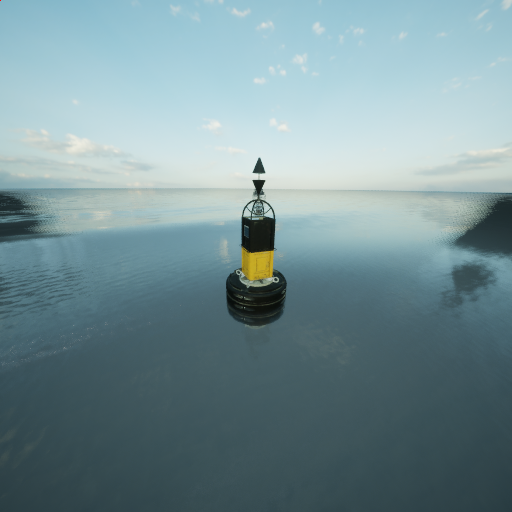
\includegraphics[width=\linewidth]{Images/BP_CM_East_15536.png}
    \caption{Image of a marker buoy generated with Unreal Engine 5}
    \label{fig:image2}
  \end{minipage}
\end{figure}

\begin{figure}[h]
  \centering
  \begin{minipage}[b]{0.9\linewidth}
    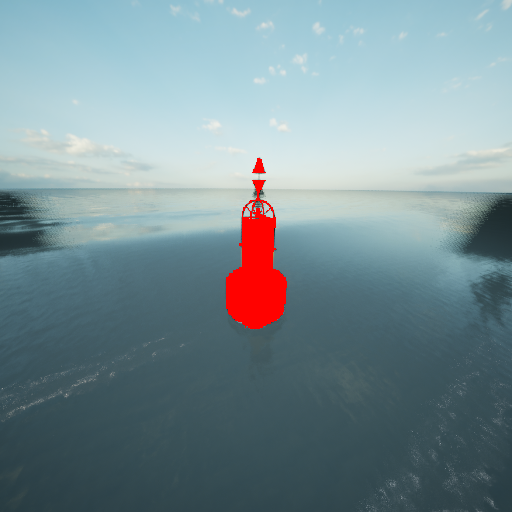
\includegraphics[width=\linewidth]{Images/BP_CM_East_15534.png}
    \caption{The same image but with a red mask applied using Unreal Engine 5's stencil system}
    \label{fig:image3}
  \end{minipage}
\end{figure}

\subsection{Arma 3}

\subsection{AI Command and Control through Decision Making}

\subsubsection{Individual Unit Approach}

\subsubsection{Alien Isolation's Alien}



\subsubsection{Mutually Supporting Units Approach}

\subsubsection{AI which can adhere to the Law of Armed Conflict}

\hl{Talk about treachery as all of the other points here seem pretty easy to program}

% https://assets.publishing.service.gov.uk/media/5f1700e7d3bf7f596d94f8de/dcdc_legal_aide_memoire_law_armed_conflict_jsp381.pdf %

\subsection{Immersive Scenarios}

An immersive scenario is one in which the \hl{user/player/trainee} is able to 'forget' that they are controlling a character in a virtual world; the less the user is immersed, the more aware they are of the reality of the situation.

\hl{Talk about those adverts where they deliberately play the game badly to make you want to take over, does this relate to people spectating in games}

% https://youtu.be/okMhLCaPuuM %
% In this video they claim Goldeneye is the first shooter game to have realistic firearms %

\hl{These are called Fail Ads} 

\subsection{Necessary Features of an Immersive Scenario}

\subsubsection{Realistic Units}

\hl{TODO: Look into whether realistic vehicles are necessary
TODO: Look into whether people can tell different things apart. Can the average person on the street tell a NATO tank apart from a Russian one? Are people's perspectives changed by WW2 films? Talk about when the girls at the beach thought that the WW2 re-enactors were recruiters and couldn't identify a uniform which was 80 years old.}

\hl{TODO: According to a study which I completed called... }

\hl{TODO: Source? Says who?}

\subsection{Audio and Visuals}

Audio and visual work to confirm the content of each other to the observer \cite{diegeticSounds1}. 

\subsubsection{Audio}

\subsubsection{Diegetic Sounds for Atmosphere}

 \cite{diegeticSounds1}

% Talk about A Plague Tale's audio "

% Talk about that game where the players thought one weapon must be better because of its sound but the stats were the same %

Wolfenstein: Enemy Territory

% https://www.youtube.com/watch?v=RDxiuHdR_T4&ab_channel=PeopleMakeGames %

"The general consensus was that if you had a Thompson, it was slower but harder hitting and if you had an MP40 it was faster but it was waker." - 1

"Uhh the Thompson was sort of like this more boxy, smaller, it sort of had like a I dunno a sturdier kind of feel to it." - 2

"You'd use it until you couldn't then begrudgingly get the MP40" - 3

\subsubsection{Visuals}

"often identical and lack the same indications of individuality as
the heroes’ avatars"

\hl{Talk about how in games with enemies, often the most difficult fight and more meaningful fight is against the one who you know and have met.
For example, generic bad guy number 1, who cares but talk about the boss fights in Grand Theft Auto or Star Wars.}

%https://journals.sagepub.com/doi/10.1177/1750635213494129%

% Talk about Bodycam the game, talk about Unrecord the game %

\subsection{Unfair Training Causing Frustration Instead of Progression}

% Talk about Call to Arms and its units spawning off map %

\subsection{Data Analysis for Performance Review}

\hl{TODO:} 

\hl{- Add a source for how counter-battery is trained using radar}

The nature of simulations is such that vast amounts of data can be collected and subsequently analysed in a way which isn't possible in real world scenarios. Although technology exists for collecting and analysing data in real-world scenarios, the sheer flexibility of simulated data is not yet matched.

For example, data regarding the source of indirect fire, such as artillery and mortars shells, can be collected and analysed by technology such as \hl{Radar, Field Artillery, No. 15} (Cymbeline). The purpose of this system is to determine the origin of the indirect fire, based on information sourced through determining the shell's velocity and trajectory. This information can then be relayed to friendly elements for use in the counter-battery role.

In the context of training for the counter-battery role as a field-gun crew in a live exercise, without simulation, a physical installation would be required to \hl{train on, including real projectiles being fired through the air} and further real projectiles needing to be fired at the source to determine the effectiveness of the field-gun crew's performance.

With a military simulation, these actions can all be carried out virtually, with the ability to gather instant, qualitative and quantitative data on the performance of the crew, \hl{(providing the simulation was accurate)}.

\section{AI Solutions to Problems with Training Effectiveness}

\section{Potential AI for those Solutions}

\subsection{Decision Trees}

A decision tree is a "non-parametric supervised learning algorithm, which is utilised for both classification and regression tasks" (https://www.ibm.com/topics/decision-trees)

Parts of the decision tree can be turned on and off to further increase complexity and improve behaviour - Slides part 1 from CE811

"A simple random number generator applied judiciously can produce a lot of believability"  (https://www.oreilly.com/library/view/artificial-intelligence-for/9780123747310/)

\subsubsection{Alien Isolation}

The famous alien in Alien Isolation makes use of decision trees to control the alien [Slides part 1 from CE811]. 

\subsection{Genetic Algorithms}

Genetic Algorithms provided the solution for optimising the layout of a military operations centre, as explained by Wenbi Wang in hl{"Layout optimization of a military operations center using a genetic algorithm".}

This task consisted of the optimisation of the layout of a command centre for the Canadian Armed Forces, consisting of 68 staff (likely a mix of all ranks although these details are omitted).

Genetic algorithms could provide a solution for generating ideal "atmospherics" for immersive scenarios. For example, determining which weather, time and objective combination makes for the most immersive scenario.  

\subsubsection{Fitness Functions}



\subsubsection{Evaluation Strategies}

\subsection{Proximal Policy Optimisation}

Proximal Policy Operation (PPO) is a reinforcement learning algorithm, which can be utilised for decision making in order for task completion. \cite{schulman2017proximal}

\section{Metrics}

\subsubsection{Observing Short-term Stress Levels}

Short-term stress levels can be observed through monitoring variable 

\section{Existing Studies}

%https://www.reddit.com/r/Screenwriting/comments/wkxnkh/alfred_hitchcocks_bomb_analogy/%

\section{Potential Studies}

%Potentially one of asking people to determine the video game from the real image%

%From Charlie Vickers regarding Arma tank screenshot: Desaturated colour palette, lack of life, and intimidating threat of rank moving towards makes sense of dread and lifelessness.%

%Something to do with driving tests and why they are so stressful%

\section*{Methods for Research}



\section{Simulator Sickness}

%https://kidshealth.org/en/teens/simulator-sickness.html%

\bibliographystyle{plain}
\bibliography{literaturereviewbib}{}


\end{document}